% Soubory musí být v kódování, které je nastaveno v příkazu \usepackage[...]{inputenc}

\documentclass[%        Základní nastavení
%  draft,    				  % Testovací překlad
  12pt,       				% Velikost základního písma je 12 bodů
  a4paper,    				% Formát papíru je A4
  %oneside,      			% Jednostranný tisk
    twoside,      			% Dvoustranný tisk (kapitoly a další důležité části tedy začínají na lichých stranách)
	unicode,						% Záložky a metainformace ve výsledném  PDF budou v kódování unicode
]{report}				    	% Dokument třídy 'zpráva', vhodná pro sazbu závěrečných prací s kapitolami

\usepackage[utf8]		  %	Kódování zdrojových souborů je UTF-8
	{inputenc}					% Balíček pro nastavení kódování zdrojových souborů

\usepackage{sectsty}
	%přetypuje nadpisy všech úrovní na bezpatkové, kromě \chapter, která je přenastavena zvlášť v thesis.sty
	\allsectionsfont{\sffamily}

\usepackage{graphicx} % Balíček 'graphicx' pro vkládání obrázků
											% Nutné pro vložení logotypů školy a fakulty

\usepackage[          % Balíček 'acronym' pro sazby zkratek a symbolů
	nohyperlinks				% Nebudou tvořeny hypertextové odkazy do seznamu zkratek
]{acronym}						
											% Nutné pro použití prostředí 'acronym' balíčku 'thesis'

\usepackage[
	breaklinks=true,		% Hypertextové odkazy mohou obsahovat zalomení řádku
	hypertexnames=false % Názvy hypertext. odkazů budou tvořeny nezávisle na názvech TeXu
]{hyperref}						% Balíček 'hyperref' pro sazbu hypertextových odkazů
											% Nutné pro použití příkazu 'pdfsettings' balíčku 'thesis'

\usepackage{pdfpages} % Balíček umožňující vkládat stránky z PDF souborů
                      % Nutné při vkládání titulních listů a zadání přímo
                      % ve formátu PDF z informačního systému

\usepackage{enumitem} % Balíček pro nastavení mezerování v odrážkách
  \setlist{topsep=0pt,partopsep=0pt,noitemsep} % konkrétní nastavení

\usepackage{cmap} 		% Balíček cmap zajišťuje, že PDF vytvořené `pdflatexem' je
											% plně "prohledávatelné" a "kopírovatelné"

%\usepackage{upgreek}	% Balíček pro sazbu stojatých řeckých písmem
											%% např. stojaté pí: \uppi
											%% např. stojaté mí: \upmu (použitelné třeba v mikrometrech)
											%% pozor, grafická nekompatibilita s fonty typu Computer Modern!
                      
%\usepackage{amsmath} %balíček pro sabu náročnější matematiky                 

\usepackage{dirtree}	% sazba adresářové struktury
                      % vhodné pro prezentaci obsahu elektronické přílohy (např. CD)

\usepackage[formats]{listings}	% Balíček pro sazbu zdrojových textů
\lstset{              % nastavení
%	Definice jazyka použitého ve výpisech
%    language=[LaTeX]{TeX},	% LaTeX
%	language={Matlab},		% Matlab
	language={C},           % jazyk C
    basicstyle=\ttfamily,	% definice základního stylu písma
    tabsize=2,			% definice velikosti tabulátoru
    inputencoding=utf8,         % pro soubory uložené v kódování UTF-8
		columns=fixed,  %fixed nebo flexible,
		fontadjust=true %licovani sloupcu
    extendedchars=true,
    literate=%  definice symbolů s diakritikou
    {á}{{\'a}}1
    {č}{{\v{c}}}1
    {ď}{{\v{d}}}1
    {é}{{\'e}}1
    {ě}{{\v{e}}}1
    {í}{{\'i}}1
    {ň}{{\v{n}}}1
    {ó}{{\'o}}1
    {ř}{{\v{r}}}1
    {š}{{\v{s}}}1
    {ť}{{\v{t}}}1
    {ú}{{\'u}}1
    {ů}{{\r{u}}}1
    {ý}{{\'y}}1
    {ž}{{\v{z}}}1
    {Á}{{\'A}}1
    {Č}{{\v{C}}}1
    {Ď}{{\v{D}}}1
    {É}{{\'E}}1
    {Ě}{{\v{E}}}1
    {Í}{{\'I}}1
    {Ň}{{\v{N}}}1
    {Ó}{{\'O}}1
    {Ř}{{\v{R}}}1
    {Š}{{\v{S}}}1
    {Ť}{{\v{T}}}1
    {Ú}{{\'U}}1
    {Ů}{{\r{U}}}1
    {Ý}{{\'Y}}1
    {Ž}{{\v{Z}}}1
}

%%%%%%%%%%%%%%%%%%%%%%%%%%%%%%%%%%%%%%%%%%%%%%%%%%%%%%%%%%%%%%%%%
%%%%%%      Definice informací o dokumentu             %%%%%%%%%%
%%%%%%%%%%%%%%%%%%%%%%%%%%%%%%%%%%%%%%%%%%%%%%%%%%%%%%%%%%%%%%%%%

% V tomto souboru se nastavují téměř veškeré informace, proměnné mezi studenty:
% jméno, název práce, pohlaví atd.
% Tento soubor je SDÍLENÝ mezi textem práce a prezentací k obhajobě -- netřeba něco nastavovat na dvou místech.

\usepackage[
%%% Z následujících voleb jazyka lze použít pouze jednu
  czech-english,		% originální jazyk je čeština, překlad je anglicky (výchozí)
  %english-czech,	% originální jazyk je angličtina, překlad je česky
  %slovak-english,	% originální jazyk je slovenština, překlad je anglicky
  %english-slovak,	% originální jazyk je angličtina, překlad je slovensky
%
%%% Z následujících voleb typu práce lze použít pouze jednu
  semestral,		  % semestrální práce (výchozí)
  %bachelor,			%	bakalářská práce
  %master,			  % diplomová práce
  %treatise,			% pojednání o disertační práci
  %doctoral,			% disertační práce
%
%%% Z následujících voleb zarovnání objektů lze použít pouze jednu
%  left,				  % rovnice a popisky plovoucích objektů budou zarovnány vlevo
	center,			    % rovnice a popisky plovoucích objektů budou zarovnány na střed (vychozi)
%
%%% Níže uvedený přepinač 'electronic' lze použít pro generování elektronické verze práce; pokud je aktivní, vnější a vnitřní okraj sazebního obrazce budou shodné pro liché i sudé stránky.
% Pozor, neplést si s volbou oneside/twoside!
% Pozor, pro tiskovou verzi nechejte vypnuté!
%	electronic			
]{thesis}   % Balíček pro sazbu studentských prací


%%% Jméno a příjmení autora ve tvaru
%  [tituly před jménem]{Křestní}{Příjmení}[tituly za jménem]
% Pokud osoba nemá titul před/za jménem, smažte celý řetězec '[...]'
\author[]{Jan}{Tomšej}

%%% Identifikační číslo autora (VUT ID)
\butid{256421}

%%% Pohlaví autora/autorky
% (nepoužije se ve variantě english-czech ani english-slovak)
% Číselná hodnota: 1...žena, 0...muž
\gender{0}

%%% Jméno a příjmení vedoucího/školitele včetně titulů
%  [tituly před jménem]{Křestní}{Příjmení}[tituly za jménem]
% Pokud osoba nemá titul před/za jménem, smažte celý řetězec '[...]'
\advisor[doc.\ Ing.]{Petr}{Beneš}[PhD.]

%%% Jméno a příjmení oponenta včetně titulů
%  [tituly před jménem]{Křestní}{Příjmení}[tituly za jménem]
% Pokud osoba nemá titul před/za jménem, smažte celý řetězec '[...]'
% Nastavení oponenta se uplatní pouze v prezentaci k obhajobě;
% v případě, že nechcete, aby se na titulním snímku prezentace zobrazoval oponent, pouze příkaz zakomentujte;
% u obhajoby semestrální práce se oponent nezobrazuje (jelikož neexistuje)
% U dizertační práce jsou typicky dva až tři oponenti. Pokud je chcete mít na titulním slajdu, prosím ručně odkomentujte a upravte jejich jména v definici "VUT title page" v souboru thesis.sty.
\opponent[doc.\ Mgr.]{Křestní}{Příjmení}[Ph.D.]

%%% Název práce
%  Parametr ve složených závorkách {} je název v originálním jazyce,
%  parametr v hranatých závorkách [] je překlad (podle toho jaký je originální jazyk).
%  V případě, že název Vaší práce je dlouhý a nevleze se celý do zápatí prezentace, použijte příkaz
%  \def\insertshorttitle{Zkác.\ náz.\ práce}
%  kde jako parametr vyplníte zkrácený název. Pokud nechcete zkracovat název, budete muset předefinovat,
%  jak se vytváří patička slidu. Viz odkaz: https://bit.ly/3EJTp5A
\title[Acoustic emission source localization]{Lokalizace zdrojů akustické emise}

%%% Označení oboru studia
%  Parametr ve složených závorkách {} je název oboru v originálním jazyce,
%  parametr v hranatých závorkách [] je překlad
\specialization[Automation and Measurement]{Automatizační~a~měřicí technika}

%%% Označení ústavu
%  Parametr ve složených závorkách {} je název ústavu v originálním jazyce,
%  parametr v hranatých závorkách [] je překlad
\department[Department of Control and Instrumentation]{Ústav automatizace a měřicí techniky}
%\department[Department of Biomedical Engineering]{Ústav biomedicínského inženýrství}
%\department[Department of Electrical Power Engineering]{Ústav elektroenergetiky}
%\department[Department of Electrical and Electronic Technology]{Ústav elektrotechnologie}
%\department[Department of Physics]{Ústav fyziky}
%\department[Department of Foreign Languages]{Ústav jazyků}
%\department[Department of Mathematics]{Ústav matematiky}
%\department[Department of Microelectronics]{Ústav mikroelektroniky}
%\department[Department of Radio Electronics]{Ústav radioelektroniky}
%\department[Department of Theoretical and Experimental Electrical Engineering]{Ústav teoretické a experimentální elektrotechniky}
%\department[Department of Control and IN]{Ústav telekomunikací}
%\department[Department of Power Electrical and Electronic Engineering]{Ústav výkonové elektrotechniky a elektroniky}

%%% Označení fakulty
%  Parametr ve složených závorkách {} je název fakulty v originálním jazyce,
%  parametr v hranatých závorkách [] je překlad
%\faculty[Faculty of Architecture]{Fakulta architektury}
\faculty[Faculty of Electrical Engineering and~Communication]{Fakulta elektrotechniky a~komunikačních technologií}
%\faculty[Faculty of Chemistry]{Fakulta chemická}
%\faculty[Faculty of Information Technology]{Fakulta informačních technologií}
%\faculty[Faculty of Business and Management]{Fakulta podnikatelská}
%\faculty[Faculty of Civil Engineering]{Fakulta stavební}
%\faculty[Faculty of Mechanical Engineering]{Fakulta strojního inženýrství}
%\faculty[Faculty of Fine Arts]{Fakulta výtvarných umění}
%
%Nastavení logotypu (v hranatych zavorkach zkracene logo, ve slozenych plne):
\facultylogo[logo/FEKT_zkratka_barevne_PANTONE_CZ]{logo/UTKO_color_PANTONE_CZ}

%%% Rok odevzdání práce
\graduateyear{2025}
%%% Akademický rok odevzdání práce
\academicyear{2025/26}

%%% Datum obhajoby (uplatní se pouze v prezentaci k obhajobě)
\date{11.\,11.\,1980} 

%%% Místo obhajoby
% Na titulních stránkách bude automaticky vysázeno VELKÝMI písmeny (pokud tyto stránky sází šablona)
\city{Brno}

%%% Abstrakt
\abstract[%
Překlad abstraktu
(v~angličtině, pokud je originálním jazykem čeština či slovenština; v~češtině či slovenštině, pokud je originálním jazykem angličtina)
]{%
Abstrakt práce v~originálním jazyce
}

%%% Klíčová slova
\keywrds[%
Překlad klíčových slov
(v~angličtině, pokud je originálním jazykem čeština či slovenština; v~češtině či slovenštině, pokud je originálním jazykem angličtina)
]{%
Klíčová slova v~originálním jazyce
}

%%% Poděkování
\acknowledgement{%
Rád bych poděkoval vedoucímu bakalářské/diplomové/disertační práce
panu Ing.~XXX YYY, Ph.D.\ za odborné vedení,
konzultace, trpělivost a~podnětné návrhy k~práci.
}%  % do tohoto souboru doplňte údaje o sobě, druhu práce, názvu...

%%%%%%%%%%%%%%%%%%%%%%%%%%%%%%%%%%%%%%%%%%%%%%%%%%%%%%%%%%%%%%%%%%%%%%%%

%%%%%%%%%%%%%%%%%%%%%%%%%%%%%%%%%%%%%%%%%%%%%%%%%%%%%%%%%%%%%%%%%%%%%%%%
%%%%%%     Nastavení polí ve Vlastnostech dokumentu PDF      %%%%%%%%%%%
%%%%%%%%%%%%%%%%%%%%%%%%%%%%%%%%%%%%%%%%%%%%%%%%%%%%%%%%%%%%%%%%%%%%%%%%
%% Při načteném balíčku 'hyperref' lze použít příkaz '\pdfsettings':
\pdfsettings
%  Nastavení polí je možné provést také ručně příkazem:
%\hypersetup{
%  pdftitle={Název studentské práce},    	% Pole 'Document Title'
%  pdfauthor={Autor studenstké práce},   	% Pole 'Author'
%  pdfsubject={Typ práce}, 						  	% Pole 'Subject'
%  pdfkeywords={Klíčová slova}           	% Pole 'Keywords'
%}
%%%%%%%%%%%%%%%%%%%%%%%%%%%%%%%%%%%%%%%%%%%%%%%%%%%%%%%%%%%%%%%%%%%%%%%

\pdfmapfile{=vafle.map}

%%%%%%%%%%%%%%%%%%%%%%%%%%%%%%%%%%%%%%%%%%%%%%%%%%%%%%%%%%%%%%%%%%%%%%%
%%%%%%%%%%%       Začátek dokumentu               %%%%%%%%%%%%%%%%%%%%%
%%%%%%%%%%%%%%%%%%%%%%%%%%%%%%%%%%%%%%%%%%%%%%%%%%%%%%%%%%%%%%%%%%%%%%%
\begin{document}
\pagestyle{empty} %vypnutí číslování stránek

%%% Vložení desek -- od září 2021 na žádost fakulty nepoužíváno
%\includepdf[pages=1]%  buďto generovaných informačním systémem
  %{pdf/student-desky}% název souboru nesmí obsahovat mezery!
%%% NEBO vytvoření desek z balíčku
%%\makecover
%%%
%\oddpage % při dvojstranném tisku přidá prázdnou stránku
%% kazdopádně ale:
%\setcounter{page}{1} %resetovaní čítače stránek -- desky do číslování nezahrnujeme

%% Vložení titulního listu
\includepdf[pages=1]%    buďto generovaného informačním systémem
  {pdf/student-titulka}% název souboru nesmí obsahovat mezery!
%% NEBO vytvoření titulní stránky z balíčku
%\maketitle
%%
\oddpage  % při dvojstranném tisku se přidá prázdná stránka
   
%% Vložení zadání
\includepdf[pages=1]%   buďto generovaného informačním systémem
  {pdf/student-zadani}% název souboru nesmí obsahovat mezery!
%% NEBO lze vytvořit prázdný list příkazem ze šablony
%\patternpage{}%
%	{\sffamily\Huge\centering ZDE VLOŽIT LIST ZADÁNÍ}%
%	{\sffamily\centering Z~důvodu správného číslování stránek}
%%
\oddpage% při dvojstranném tisku se přidá prázdná stránka

%% Vysázení stránky s abstraktem
\makeabstract

% Vysázení stránky s rozšířeným abstraktem
% (pokud píšete práci v češtině či slovenštině, vložení rozšířeného abstraktu zrušte;
%  pro semestrální projekt také není potřeba rozšířený abstrakt uvádět)
% Vysázení stránky s rozšířeným abstraktem
% (týká se pouze bc. a dp. prací psaných v angličtině, viz Směrnice rektora 72/2017)
\cleardoublepage
\noindent
{\large\sffamily\bfseries\MakeUppercase{Rozšířený abstrakt}}
\\
Výtah ze směrnice rektora 72/2017:\\
\emph{Bakalářská a diplomová práce předložená v angličtině musí obsahovat rozšířený abstrakt v češtině
nebo slovenštině (čl. 15). To se netýká studentů, kteří studují studijní program akreditovaný v
angličtině.}
(čl. 3, par. 7)\\
\emph{Nebude-li vnitřní normou stanoveno jinak, doporučuje se rozšířený abstrakt o rozsahu přibližně 3
normostrany, který bude obsahovat úvod, popis řešení a shrnutí a~zhodnocení výsledků.}
(čl. 15, par. 5)

%%% Vysázení citace práce
\makecitation

%%% Vysázení prohlášení o samostatnosti
\makedeclaration

%%% Vysázení poděkování
\makeacknowledgement

%%% Vysázení obsahu
\tableofcontents

%%% Vysázení seznamu obrázků
% (vynechejte, pokud máte dva nebo méně obrázků)
\listoffigures

%%% Vysázení seznamu tabulek
% (vynechejte, pokud máte dvě nebo méně tabulek)
\listoftables

%%% Vysázení seznamu výpisů kódu
% (vynechejte, pokud máte dva nebo méně výpisů)
\lstlistoflistings

\cleardoublepage\pagestyle{plain}   % zapnutí číslování stránek

%Pro vkládání kapitol i příloh používejte raději \include než \input
%%% Vložení souboru 'text/uvod.tex' s úvodem
\chapter*{Úvod}
\phantomsection
\addcontentsline{toc}{chapter}{Úvod}


Úvod studentské práce, např\,\dots

Nečíslovaná kapitola Úvod obsahuje \uv{seznámení} čtenáře s~problematikou práce.
Typicky se zde uvádí:
(a) do jaké tematické oblasti práce spadá, (b) co jsou hlavní cíle celé práce a (c) jakým způsobem jich bylo dosaženo.
Úvod zpravidla nepřesahuje jednu stranu.
Poslední odstavec Úvodu standardně představuje základní strukturu celého dokumentu.

Tato práce se věnuje oblasti \acs{DSP} (\acl{DSP}), zejména jevům, které nastanou při nedodržení Nyquistovy podmínky pro \ac{symfvz}.%
\footnote{Tato věta je pouze ukázkou použití příkazů pro sazbu zkratek.}

Šablona je nastavena na \emph{dvoustranný tisk}.
Nebuďte překvapeni, že ve vzniklém PDF jsou volné stránky.
Je to proto, aby důležité stránky jako např.\ začátky kapitol začínaly po vytisknutí a svázání vždy na pravé straně.
%
Pokud máte nějaký závažný důvod sázet (a~zejména tisknout) jednostranně, nezapomeňte si přepnout volbu \texttt{twoside} na \texttt{oneside}!

%%% Vložení souboru 'text/cile.tex' s úvodem
\chapter*{Cíle práce}
\phantomsection
\addcontentsline{toc}{chapter}{Cíle práce}

Konkrétní specifikace cílů, které má autor v~práci vyřešit.
Tato kapitola je \emph{volitelná} -- pokud váš studijní program nevyžaduje zvláštní kapitolu s cíli,
cíle specifikujte v~rámci Úvodu.

%%% Vložení souboru 'text/reseni' s popisem řešení práce
% (rozdělte na více souborů či kapitol, pokud je vhodné)
\chapter{Úvod do problematiky testování materiálů, metody vlastního testování, metoda akustické emise}

\section{Nedestruktivní testování}
V technické praxi jsou struktury namáhány mnoha vnějšími vlivy, čímž se mění jejich materiálové vlastnosti. Například, u laminátových kontrukcí v leteckém průmyslu může vlivem sil nárazu pevnost v tlaku klesnout až o 80\%, i když se materiál jeví jako nepoškozený \cite{Benes_podklad_advances}. 

Pro posouzení stavu materiálu je proto nutné provádět pravidelné testování.
Za účelem stanovení mezních vlastností materiálu jako pevnosti v tlaku, pevnosti v~tahu, lomové houževnatosti, atd., bývá prováděno \ac{DT}. Zahrnuje např. zkoušku tahem, tlakem, nebo ohybem. K těmto zkouškám jsou používány speciální stroje – kladiva, trhačky, ohýbačky, aj. Jak je z názvu přímo patrné, vlastní destruktivní zkoušení končí nevratným poškozením vzorku. 

Pro již hotové konstrukce (např. svařované konstrukce v zámečnické výrobě, betonové pilíře v oblasti stavebnictví) nebo komponenty (hřídele, ozubená kola, kolejnice, atd.) se metody \ac{DT} zpravidla nepoužívají, jelikož by takové zkoušení bylo příliš nákladné. Nabízí se proto použití metod \ac{NDT}. Počátky \ac{NDT} sahají do 19. století, kdy pomocí tzv. akustického poklepového testování byly detekovány praskliny na železničních kolech \cite{ConcretetestingHELAL}.
\section{Metody nedestruktivního testování}
Velká výhoda metod \ac{NDT} spočívá v možnosti zkoušení v kterékoliv části životního cyklu produktu, u některých metod dokonce i v průběhu vykonávání vlastní činnosti výrobku. Díky tomu dostáváme přesné informace o poloze a závažnosti případného defektu ve struktuře materiálu. V současné době na trhu dominuje pět metod nedestruktivního testování – zkoušení magnetickými částicemi, radiografické zkoušení, ultrazvukové zkoušení, zkoušení vířivými proudy a zkoušení metodou akustické emise (dále AE).

Zkoušení magnetickými částicemi spočívá ve vystavení feromagnetických materiálů magnetickému poli. Díky vysoké permeabilitě feromagnetického materiálu se magnetické domény orientují ve~směru působení magnetického pole, tvoří tak souvislé čáry. V případě nespojitosti materiálu dojde k tzv. úniku magnetického pole – čáry v~bodě defektu nebudou spojité. Pro~snadnou viditelnost těchto nespojitostí je použit prášek oxidu železitého, který zmíněné čáry a nespojitosti kopíruje \cite{Gupta_ADVANCES_IN_MATERIALS_AND_PROCESSING_TECHNOLOGIES}. Mezi~limity spadá možnost použití jen pro feromagnetické materiály (železo, kobalt, nikl, ferity, gadolinium, aj.) \cite{Sandeep_Kumar_Dwivedi_NDT}.

Radiografické zkoušení je postup založen na snímání obrázků s využitím radioaktivního zdroje záření. Záření je pohlcováno materiálem a dochází tak k útlumu. Defekty na těchto snímcích lze rozpoznat jako místa s menším útlumem záření \cite{Gupta_ADVANCES_IN_MATERIALS_AND_PROCESSING_TECHNOLOGIES}. Limity představuje nutnost radiační ochrany a nevhodnost použití pro porézní materiály (např. beton, dřevo, sádra, keramiky, kosti aj.) \cite{Sandeep_Kumar_Dwivedi_NDT}

Při zkoušení ultrazvukem je používáno zvukových vln. Piezoelektrický snímač generuje pulzy, které se šíří materiálem. Cestují-li tyto pulzy nepoškozenou, spojitou strukturou, nemění se jejich parametry (především tedy rychlost). Při defektu dochází ke změně rychlosti pulzů.\cite{Gupta_ADVANCES_IN_MATERIALS_AND_PROCESSING_TECHNOLOGIES}. 

Během zkoušení vířivými proudy je kovový materiál umístěn do fluktuujího magnetického pole, které je vytvářeno cívkou. V kovovém materiálu jsou indukovány proudy s vířivou povahou (proto vířivé proudy). Těmito vířivými proudy je vytvořeno sekundární magnetické pole, které ovlivňuje pole cívky. S defektem ve struktuře materiálu dojde tedy ke změně i vířivých proudů, což ovlivní i primární magnetické pole cívky \cite{Gupta_ADVANCES_IN_MATERIALS_AND_PROCESSING_TECHNOLOGIES}. 
\section{Metoda AE. Její výhody, limity}
V případě, že je kovový materiál deformován, uvolňuje se energie ve formě tzv. elastických vln. Tyto elastické vlny jsou vlny vysoké frekvence, které cestují směrem k~povrchu materiálu. Na povrchu tato data sbírají snímače AE. Souřadnice zdrojů AE jsou nejčastěji stanovovány pomocí známého triangulačního algoritmu (podle normy ČSN 14584 \cite{čsn14584}) dle časových diferencí příchodů signálů k jednotlivým snímačům. Tyto snímače jsou na zkoušeném vzorku umístěny v husté síti.

Oproti ultrazvukovému testování je velkou výhodou zkoušení AE možnost nepřetržitého monitorování komponent – při ultrazvukovém zkoušení je potřeba externí zdroj zvuku o vysoké frekvenci. Metodou \ac{AE} se kromě toho nabízí testovat i nekovové nebo porézní materiály a najde tak uplatnění i v netechnických a medicínských oborech (např. diagnostika kostí a kloubů v ortopedii).

Limit metody AE spočívá hlavně v interpretaci dat u komplikovanějších struktur~–~analytické vzorce pro lokalizace zdrojů AE jsou známé jen pro tenkou, izotropní desku \cite{Chlada2009}. Navíc, instalace senzorů na všech požadovaných místech je mnohdy nesnadná. Může tomu tak být z důvodu nepřístupnosti do určitých lokalit konstrukcí (např. některé koutové sváry). Umístění snímačů dokáže mimo to nežádoucím způsobem ovlivnit dynamické vlastnosti konstrukce. %U složitějších struktur probíhá snaha uplatnit umělou neuronovou síť ke zpracování dat.
\section{Postupy použití metody AE u složitějších struktur}%Kompenzace limitů metody AE} 
Z pohledu systémové teorie můžeme testování materiálů metodou AE formulovat dvěma základními způsoby; při~\textbf{dopředné úloze} je stanovována odezva dle známých vstupů (sil nárazů). Nelze-li snadno získat hodnotu vstupu, je formulován problém zpětný – ze~změřené odezvy se dopočítávají hodnoty vstupů. Tento způsob řešení nazveme \textbf{inverzním algoritmem}.

Ve vědeckých studiích bývají tyto inverzní algoritmy k~rekonstrukci působení vnějších sil hojně využívány. Podle implementace již zmíněné inverzní algoritmy jde rozdělit na~techniky založené na~modelech a~techniky založené na~strojovém/hlubokém učení.
\subsection{Techniky založené na modelech}
Při~testování materiálu je odezva (signál AE) zpracovaná předem~vytvořeným modelem. Tento model dle~zpracované odezvy stanovuje vstupní hodnotu a~následně polohu nespojitosti materiálu. Výhoda této techniky spočívá v~nízké výpočetní náročnosti. V používání limituje nutnost tvorby přesného modelu pro přepočty – jak již~bylo výše uvedeno, pro~stanovení vad u~komplikovanějších anizotropních materiálů nejsou známé analytické vzorce, a~je proto velmi obtížné tvořit modely pro testování těchto materiálů. Proto probíhá snaha uplatnit při lokalizaci zdrojů \ac{AE} algoritmy strojového učení.
\subsection{Techniky založené na strojovém učení}
V posledních letech se algoritmy strojového učení stávají velmi vhodnými při~rekonstrukci dat AE – dají se aplikovat i tehdy, když základní mechanismy pro nás nejsou zcela známé a nedovedeme tak správně sestavit model. Nicméně, pro správné uplatnění technik strojového učení představuje omezení nutnost velkého objemu tréninkových dat. 

Neexistuje žádná záruka, že tréninková data získaná pro jednu strukturu přinesou smysluplné výsledky i u struktur odlišných. V posledních letech jsou prozkoumávány proto metody tzv. hlubokého učení (nebo také deep learningu), které umožňují použití dat i v surové podobě. S použitím metod hlubokého učení lze tak interpretovat dokonce i vícerozměrné signály \ac{AE}.

Důležitým algoritmem, na kterém stojí velká většina modelů hlubokého učení, je \textbf{umělá neuronová síť}. Stejně jako ostatní metody hlubokého učení potřebují ke své funkci velký objem tréninkových dat. Studie (například \cite{ghajari}) se v současné době snaží pomocích neuronových sítí identifikovat vnější síly, které způsobují deformační změny na kompozitních panelech. Výhodou neuronových sítí je nepotřeba předchozích znalostí poloh zdrojů deformace. Ve výše uvedené studii jsou aplikovány dvě neuronové sítě – jedna pro deformace o vyšších amplitudách, druhá pro deformace o amplitudách menších.

Navzdory obrovskému potenciálu nejsou umělé neuronové sítě v nelineárních strukturách zcela široce využívány. Způsobují to fakta, že nejčastěji používaná architektura umělých neuronových sítí pracuje s dvourozměrnými vstupy. Prvním parametrem je rozsah datového setu, který je k dispozici k trénování sítě. Druhým je samotný příznak čili měřená data, která neuronové síti přidělíme k učení. Tyto parametry nezahrnují čas, jenž je k rekonstrukci zdroje deformace nezbytný.

Navíc, pro výběr kvalitních příznaků do učící sady je nezbytná lidská expertíza. Tvorba učící sady je poměrně náročná a nelze ji nijak efektivně automatizovat. Při rekonstrukci zdroje deformace mimo jiné představuje problém již výše popsaný u technik založených na modelech – pro získání kvalitních dat je nutné rozmístit senzory v husté síti, a to zhoršuje dynamické parametry konstrukce.

\section{Komerční použití neuronových sítí pro lokalizaci AE}
AE bývá někdy označována jako pasivní ultrazvuk. Ultrazvukové snímače oproti snímačům AE potřebují pro správnou lokalizaci zdroj zvuku o frekvenci, která je vyšší než hranice slyšitelná člověkem (přes 20 kHz). Proto se mnozí výrobci ultrazvukových snímačů a defektoskopů úzce specializují i na diagnostiku metodou AE (např. Olympus). 

Velkým výrobcem, který je kromě jiných metod zaměřen i na AE, je MISTRAS group (patří k nim Physical Acoustic). Menší firma vyrábějící kvalitní a uznávané systémy, snímače a předzesilovače pro testování metodou AE, je Vallen Systeme. Jde tak o velkého konkurenta firmy MISTRAS group. Tito dva největší výrobci mimo jiné ladí a vyvíjejí software pro lokalizaci zdrojů AE pomocí algoritmů neuronových sítí.

% MISTRAS group je provozovatelem všech výše zmíněných metod \ac{DT} – věnují se jak ultrazvukovému testování, testování magnetickými částicemi, i zkoušení materiálů vířivými proudy. Pro testování metodou \ac{AE} provozují vlastní technologickou divizi Physical acoustic. 

%NA ZÁKLADĚ ZPRÁV Z VALLENA A MISTRAS POSOUDIT NÁSLEDUJÍCÍ BODY:
%JAKOU LOKALIZACI ZDROJŮ NABÍZEJÍ (CO 2D/3D DATA)?
%S JAKOU MINIMÁLNÍ VZDÁLENOSTÍ PENTESTU OD SNÍMAČE SE POČÍTÁ?
%JAKÉ TYPY VLN ZVLÁDAJÍ VYHODNOCOVAT?
%//
% Nejnovější generace 32bitového software od společnosti Vallen Systeme pro Windows k analýze zdrojů \ac{AE} se nazývá VisualAE. Součástí tohoto softwaru je stejně tak VisualClass (systém pro tzv. rozpoznávání vzorů) a VisualTR (modul pro digitální filtraci signálu). Veškerá data jsou sbírána podprogramem Acquisition32, který má vysokou spolehlivost a je plně integrován do tohoto systému. Jak VisualClass, tak VisualAE, a stejně tak i VisualTR se tak mohou kdykoliv dostat k libovolnému datasetu.
\subsection{Software od firmy Vallen}
Program VisualClass od společnosti Vallen
 umí rozeznat podobnosti a rozdíly 
 mezi změřenými vlnami AE. Jak je z názvu přímo patrné, umí tato data klasifikovat~–~každé vlně přidělí určité číslo třídy. V každé z těchto přidělených tříd klasifikuje podobnost se vzorovými 
daty. Funkcí, která představuje míru podobnosti mezi vlastní změřenou vlnou a vzorem, je poměr vzdáleností. Čím nižší je poměr vzdáleností, tím lépe odpovídá aktuální průběh přidělené třídě. Výsledky těchto klasifikátorů mohou být pro každý dílčí detekovaný zásah v programu VisualAE (program od společnosti Vallen pro analýzu dat AE. Zpracovává jak dvojrozměrná, tak trojrozměrná data, počítá hodnoty nejistot měření, atd.) spojeny s odpovídajícími parametry. Klasifikované výsledky lze tak i statisticky zpracovat.

Výše zmíněný klasifikátor (čili kritérium, kterým jsou vlnové průběhy přidělovány do tříd) lze chápat jako výsledek procesu učení. V rámci procesu učení je brán určitý počet datových (učících) sad. Byla-li data vybrána uživatelem, hovoří se o \textbf{řízeném učení} (supervised learning). Pokud byly tyto sady vybrány automaticky nějakým výkonným algoritmem shlukování (tzv. clustering), jde potom o učení \textbf{neřízené} (unsupervised learning).

Průběhy uvedené na obrázcích \ref{fig:visualclass_3cm}, \ref{fig:visualclass_6cm} a \ref{fig:visualclass_11cm} byly změřeny shodným senzorem, zpracování proběhlo softwarem od VisualClass. Vzdálenost zdroje AE od snímače jsou 3, 6 a 11 cm. Pro každou z níže uvedených pozic bylo generováno deset pulzů.
\begin{figure}[!h]
    \centering
    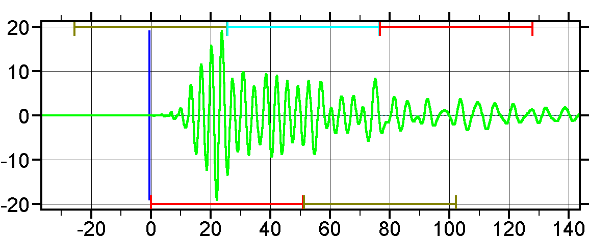
\includegraphics[width=0.7\linewidth]{obrazky/visualclass_3cm.png}
    \caption{Signál akustické emise pro vzdálenost senzoru od zdroje 3 cm \cite{vallen_visual_class}}
    \label{fig:visualclass_3cm}
\end{figure}

\begin{figure}[!h]
    \centering
    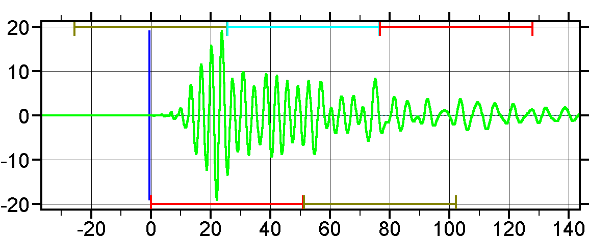
\includegraphics[width=0.7\linewidth]{obrazky/visualclass_3cm.png}
    \caption{Signál akustické emise pro vzdálenost senzoru od zdroje 6 cm \cite{vallen_visual_class}}
    \label{fig:visualclass_6cm}
\end{figure}

\begin{figure}[!h]
    \centering
    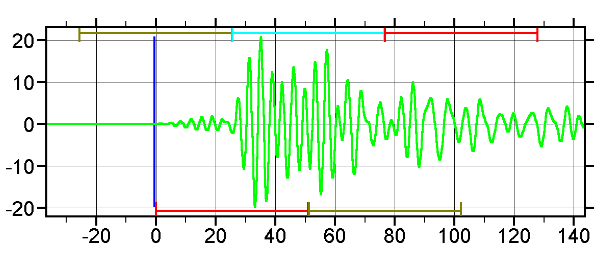
\includegraphics[width=0.7\linewidth]{obrazky/visualclass_11cm.png}
    \caption{Signál akustické emise pro vzdálenost senzoru od zdroje 11 cm \cite{vallen_visual_class}}
    \label{fig:visualclass_11cm}
\end{figure}
Pro takto změřené signály
 AE potom VisualClass dokáže zobrazovat 
 spektra krátkodobé frekvenční analýzy 
 (zobrazení spektrogramu). 
 Příklad frekvenční analýzy pro průběh uvedený na~obrázku \ref{fig:visualclass_3cm} je uveden na~obrázku \ref{fig:vallen_frekvencni_analyza}. 
\begin{figure}[!h]
    \centering
    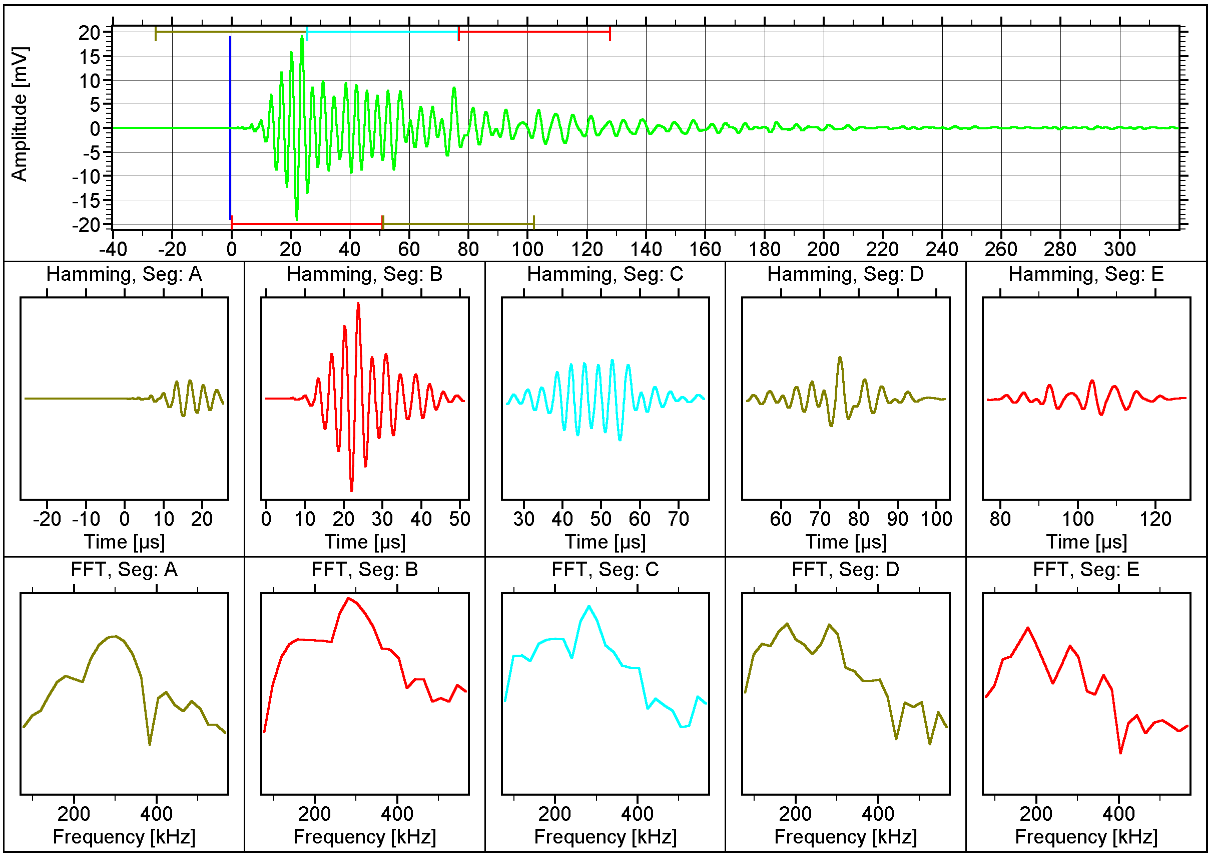
\includegraphics[width=0.75\linewidth]{visual_class_spectral_analysis.png}
    \caption{Frekvenční analýza pro signál AE z obrázku \ref{fig:visualclass_3cm} \cite{vallen_visual_class}}
    \label{fig:vallen_frekvencni_analyza}
\end{figure}
Jak lze na obrázku 
\ref{fig:vallen_frekvencni_analyza} vidět, 
je signál rozdělen na~malé časové segmenty. 
Každý z těchto časových segmentů je zobrazen 
pomocí Hammingova okna, abychom se 
vyhnuli strmým hranám oken. 
Tyto hrany totiž zkreslují skutečné průběhy.
Následně se pro každý v horní části
obrázku \ref{fig:vallen_frekvencni_analyza} 
vyznačený časový segment
pomocí algoritmu FFT stanoví vlastní spektrum, 
jak lze vidět ve spodní části obrázku 
\ref{fig:vallen_frekvencni_analyza}.

Počet časových segmentů, počet 
vzorků na segment nebo rozsah harmonických,
jsou parametry nastavitelné uživatelem společně 
se~stovkami dalších funkcí pro signálové operace.
Jak dobře změřený signál a jeho vlastnosti odpovídají
vzoru, udávají tzv. Fischerovy poměry. 
Sledované vlastnosti lze vybrat přímo, nebo 
automaticky. Na obrázku \ref{fig:vallen_fisherovy_vzorce}
vidíme příklad těchto poměrů, kde červené tečky
představují klasifikátor, se kterým se právě pracuje.
\begin{figure}[!h]
    \centering
    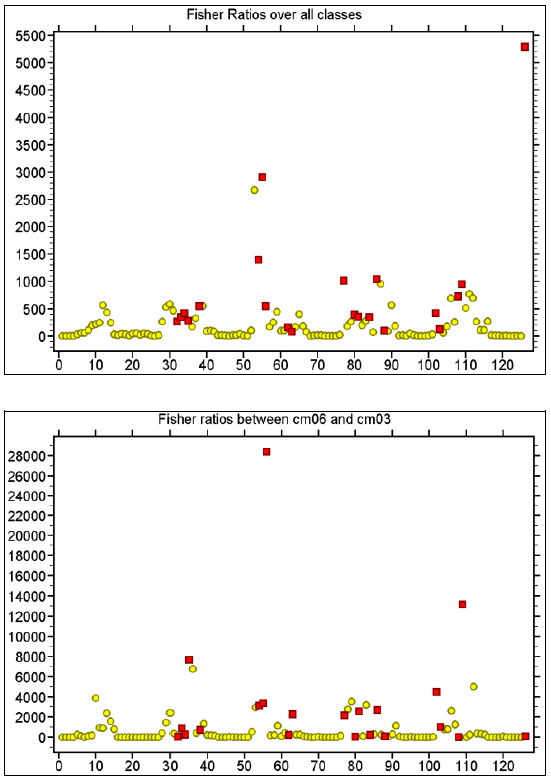
\includegraphics[width=0.75\linewidth]{obrazky/visual_class_fisher_ratios.png}
    \caption{Fisherovy poměry pro všechny třídy (nahoře), pro vybrané třídy (dole) \cite{vallen_visual_class}}
    \label{fig:vallen_fisherovy_vzorce}
\end{figure}

Působivou utilitou softwaru VisualClass pro srovnávání
několika naměřených průběhů navzájem mezi sebou je 
schopnost tzv. feature-feature projekce.
Každý~změřený průběh AE patřící k jedné třídě 
značí barevný symbol. Díky tomuto zobrazení lze 
snadno ověřit rozdíly jak mezi signály stejné třídy, 
tak mezi několika třídami. Zobrazení tzv. feature-feature demonstruje 
obrázek \ref{fig:vallen_feature_feature}
\begin{figure}[!h]
    \centering
    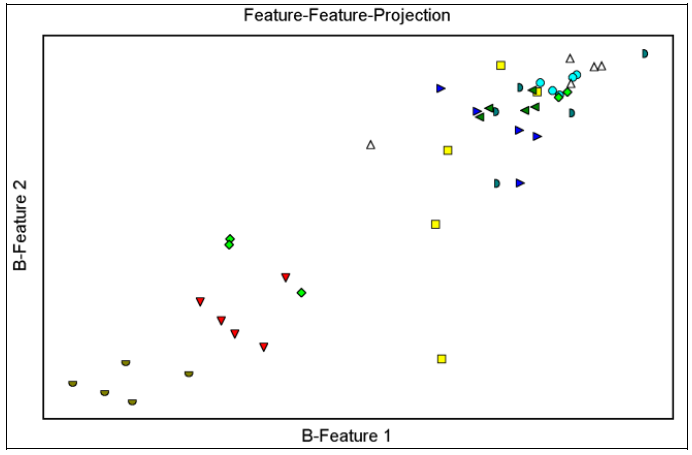
\includegraphics[width=0.75\linewidth]{obrazky/visual_class_feature_feature.png}
    \caption{Fisherovy poměry pro všechny třídy (nahoře), pro vybrané třídy (dole) \cite{vallen_visual_class}}
    \label{fig:vallen_feature_feature}
\end{figure}
\subsection{Software od firmy Physical acoustic (MISTRAS)}

\section{Případný vývoj}









%%% Vložení souboru 'text/vysledky' s popisem vysledků práce
% (rozdělte na více souborů či kapitol, pokud je vhodné)
\chapter{Výsledky studentské práce}

Praktická část a výsledky studentské práce vhodně rozdělené do částí.

\section{Programové řešení}

%Aliquam ante. Phasellus faucibus molestie nisl. Etiam ligula pede, sagittis quis, interdum ultricies, scelerisque eu. Morbi leo mi, nonummy eget tristique non, rhoncus non leo. Cum sociis natoque penatibus et magnis dis parturient montes, nascetur ridiculus mus. Morbi scelerisque luctus velit. Curabitur bibendum justo non orci. Donec quis nibh at felis congue commodo. Nullam faucibus mi quis velit. Aenean id metus id velit ullamcorper pulvinar. Pellentesque sapien. Fusce nibh. Vestibulum fermentum tortor id mi. Nullam eget nisl. Praesent vitae arcu tempor neque lacinia pretium. Proin in tellus sit amet nibh dignissim sagittis. Donec quis nibh at felis congue commodo.
%
%Nam quis nulla. Proin in tellus sit amet nibh dignissim sagittis. Nullam dapibus fermentum ipsum. Curabitur ligula sapien, pulvinar a vestibulum quis, facilisis vel sapien. Nam libero tempore, cum soluta nobis est eligendi optio cumque nihil impedit quo minus id quod maxime placeat facere possimus, omnis voluptas assumenda est, omnis dolor repellendus. Vivamus ac leo pretium faucibus. Nunc tincidunt ante vitae massa. Maecenas sollicitudin. Ut tempus purus at lorem. Nullam lectus justo, vulputate eget mollis sed, tempor sed magna. Fusce consectetuer risus a nunc. Etiam quis quam.
%
%Donec quis nibh at felis congue commodo. Sed vel lectus. Donec odio tempus molestie, porttitor ut, iaculis quis, sem. Nullam feugiat, turpis at pulvinar vulputate, erat libero tristique tellus, nec bibendum odio risus sit amet ante. Sed elit dui, pellentesque a, faucibus vel, interdum nec, diam. Cras elementum. Sed vel lectus. Donec odio tempus molestie, porttitor ut, iaculis quis, sem. Etiam neque. Integer tempor. Vivamus porttitor turpis ac leo. Nulla non arcu lacinia neque faucibus fringilla.
%
%Etiam posuere lacus quis dolor. Nemo enim ipsam voluptatem quia voluptas sit aspernatur aut odit aut fugit, sed quia consequuntur magni dolores eos qui ratione voluptatem sequi nesciunt. Nullam faucibus mi quis velit. Cum sociis natoque penatibus et magnis dis parturient montes, nascetur ridiculus mus. Phasellus faucibus molestie nisl. Maecenas ipsum velit, consectetuer eu lobortis ut, dictum at dui. Maecenas aliquet accumsan leo. Pellentesque ipsum. Donec vitae arcu. Suspendisse nisl. Morbi imperdiet, mauris ac auctor dictum, nisl ligula egestas nulla, et sollicitudin sem purus in lacus. Pellentesque ipsum. Ut enim ad minima veniam, quis nostrum exercitationem ullam corporis suscipit laboriosam, nisi ut aliquid ex ea commodi consequatur? Nam libero tempore, cum soluta nobis est eligendi optio cumque nihil impedit quo minus id quod maxime placeat facere possimus, omnis voluptas assumenda est, omnis dolor repellendus.


%%% Vložení souboru 'text/zaver' se závěrem
\chapter*{Závěr}
\phantomsection
\addcontentsline{toc}{chapter}{Závěr}

Shrnutí studentské práce.


%%% Vložení souboru 'text/literatura' se seznamem zdrojů
% Pro sazbu seznamu literatury použijte jednu z následujících možností

%%%%%%%%%%%%%%%%%%%%%%%%%%%%%%%%%%%%%%%%%%%%%%%%%%%%%%%%%%%%%%%%%%%%%%%%%
%1) Seznam citací definovaný přímo pomocí prostředí literatura / thebibliography

\begin{thebibliography}{99}
	
\bibitem{sr72/2017}
	VYSOKÉ UČENÍ TECHNICKÉ V~BRNĚ.
	\emph{Směrnice č.\,72/2017, Úprava, odevzdávání a~zveřejňování závěrečných prací.}
	Online. Brno: VUT v~Brně, 2017.
	Úplné znění ke dni 11.\,4.\,2022.
	Dostupné z:\\
	{\small
	\url{https://www.vut.cz/uredni-deska/vnitrni-predpisy-a-dokumenty/smernice-c-72-2017-uprava-odevzdavani-a-zverejnovani-zaverecnych-praci-d161410}.}
	[cit.\ 2023-09-27].

\bibitem{CSN_ISO_690-2022}
    ÚŘAD PRO TECHNICKOU NORMALIZACI, METROLOGII A~STÁTNÍ ZKUŠEBNICTVÍ.
    ČSN ISO 690:2022 (01 0197), \emph{Informace a dokumentace -- Pravidla pro bibliografické odkazy a~citace informačních zdrojů.}
    Čtvrté vydání. Praha, 2022.

\bibitem{CSN_ISO_7144-1997}
    ÚŘAD PRO TECHNICKOU NORMALIZACI, METROLOGII A~STÁTNÍ ZKUŠEBNICTVÍ.
    ČSN ISO 7144 (010161), \emph{Dokumentace -- Formální úprava disertací a~podobných dokumentů.}
%    24 stran.
    Praha, 1997.

\bibitem{CSN_ISO_31-11}
    ÚŘAD PRO TECHNICKOU NORMALIZACI, METROLOGII A~STÁTNÍ ZKUŠEBNICTVÍ.
    ČSN ISO 31-11, \emph{Veličiny a~jednotky -- část 11: Matematické znaky a~značky používané ve fyzikálních vědách a~v~technice.}
    Praha, 1999.

\bibitem{Farkasova23:CSNISO6902022komentar}
	FARKAŠOVÁ, B.; GARAMSZEGI T.; JANSOVÁ L.; KONEČNÝ L.; KRČÁL M.\ et~al.
	\emph{Výklad normy ČSN ISO 690:2022 (01 0197) účinné od 1.\,12.\,2022}.
	 Online. První vydání. 2023.
	Dostupné~z:
	\url{https://www.citace.com/Vyklad-CSN-ISO-690-2022.pdf}.
	[cit.\,2023-09-27].



\bibitem{ConcretetestingHELAL}
    HELAL, J.; SOFI, M. a MENDIS, P. Non-Destructive Testing of Concrete: A Review of Methods. Online. 2015, roč. 2015, č. 14. Dostupné z: https://ejsei.com/EJSE/article/view/193. [cit. 2025-09-25].
\bibitem{Benes_podklad_advances.}
\bibitem{Gupta_ADVANCES_IN_MATERIALS_AND_PROCESSING_TECHNOLOGIES}
\bibitem{Sandeep_Kumar_Dwivedi_NDT}
\end{thebibliography}


%%%%%%%%%%%%%%%%%%%%%%%%%%%%%%%%%%%%%%%%%%%%%%%%%%%%%%%%%%%%%%%%%%%%%%%%%
%%2) Seznam citací pomocí BibTeXu
%% Při použití je nutné v TeXnicCenter ve výstupním profilu aktivovat spouštění BibTeXu po překladu.
%% Definice stylu seznamu
%\bibliographystyle{unsrturl}
%% Pro českou sazbu lze použít styl czechiso.bst ze stránek
%% http://www.fit.vutbr.cz/~martinek/latex/czechiso.tar.gz
%%\bibliographystyle{czechiso}
%% Vložení souboru se seznamem citací
%\bibliography{text/literatura}
%
%% Následující příkaz je pouze pro ukázku sazby literatury při použití BibTeXu.
%% Způsobí citaci všech zdrojů v souboru literatura.bib, i když nejsou citovány v textu.
%\nocite{*}

%%% Vložení souboru 'text/zkratky' se seznam použitých symbolů, veličin a zkratek
\cleardoublepage
\chapter*{\listofabbrevname}
\phantomsection
\addcontentsline{toc}{chapter}{\listofabbrevname}

\begin{acronym}[KolikMista]

	% \acro{zkTemp}		% název
	% 	[Šířka levého sloupce Seznamu symbolů a zkratek]								% zkratka
	% 	{je určena šířkou parametru prostředí \texttt{acronym} (viz řádek~1 výpisu zdrojáku na~str.\,\pageref{lst:zkratky})}
	% 										% rozvinutí zkratky

	% \acro{zkDummy}
	% 	[KolikMista]
	% 	{pouze ukázka vyhrazeného místa}

	\acro{DT}		% název/zkratka
		{destruktivní testování}
											% rozvinutí zkratky
	%%% bsymfvz
	\acro{NDT}						% název
		% [\ensuremath{f_\textind{vz}}] % symbol
		{nedestruktivní testování}					% popis
	%%% esymfvz
    \acro{AE}
    {akustická emise}
\end{acronym}


%%% Začátek příloh
\appendix

%%% Vysázení seznamu příloh
% (vynechejte, pokud máte dvě nebo méně příloh)
\listofappendices

%%% Vložení souboru 'text/prilohy' s přílohami
% Obvykle je přítomen alespoň popis co najdeme na přiloženém médiu
\chapter{Některé příkazy balíčku \texttt{thesis}}

\section{Příkazy pro sazbu veličin a jednotek}

\begin{table}[!h]
  \caption[Přehled příkazů]{Přehled příkazů pro matematické prostředí }
  \begin{center}
  	\small
	  \begin{tabular}{|c|c|c|c|}
	    \hline
	    Příkaz    						& Příklad 					& Zdroj příkladu  							& Význam  \\
	    \hline\hline
	    \verb|\textind{...}|	& $\beta_\textind{max}$ 	& \verb|$\beta_\textind{max}$|	& textový index \\
	    \hline
	    \verb|\const{...}| 		& $\const{U}_\textind{in}$ 				& \verb|$\const{U}_\textind{in}$|		& konstantní veličina \\
	    \hline
	    \verb|\var{...}| 		& $\var{u}_\textind{in}$ & \verb|$\var{u}_\textind{in}$| & proměnná veličina \\
	    \hline
	    \verb|\complex{...}| 	& $\complex{u}_\textind{in}$ & \verb|$\complex{u}_\textind{in}$| & komplexní veličina \\
	    \hline
	    \verb|\vect{...}| 		& $\vect{y}$ 						& \verb|$\vect{y}$| & vektor \\
	    \hline
	    \verb|\mat{...}| 	& $\mat{Z}$ 						& \verb|$\mat{Z}$| & matice \\
	    \hline
	    \verb|\unit{...}| 		& $\unit{kV}$ 						& \verb|$\unit{kV}$|\quad či\ \, \verb|\unit{kV}| & jednotka \\
	    \hline
	  \end{tabular}
  \end{center}
\end{table}



%\newpage
\section{Příkazy pro sazbu symbolů}

\begin{itemize}
  \item
    \verb|\E|, \verb|\eul| -- sazba Eulerova čísla: $\eul$,
  \item
    \verb|\J|, \verb|\jmag|, \verb|\I|, \verb|\imag| -- sazba imaginární jednotky: $\jmag$, $\imag$,
  \item
    \verb|\dif| -- sazba diferenciálu: $\dif$,
  \item
    \verb|\sinc| -- sazba funkce: $\sinc$,
  \item
    \verb|\mikro| -- sazba symbolu mikro stojatým písmem%
			\footnote{znak pochází z~balíčku \texttt{textcomp}}: $\mikro$,
	\item
		\verb|\uppi| -- sazba symbolu $\uppi$
			(stojaté řecké pí, na rozdíl od \verb|\pi|, což sází $\pi$).
\end{itemize}
%
Všechny symboly jsou určeny pro matematický mód, vyjma \verb|\mikro|, jenž je\\ použitelný rovněž v~textovém módu.
%$\upmikro$


\chapter{Druhá příloha}

\begin{figure}[!h]
  \begin{center}
    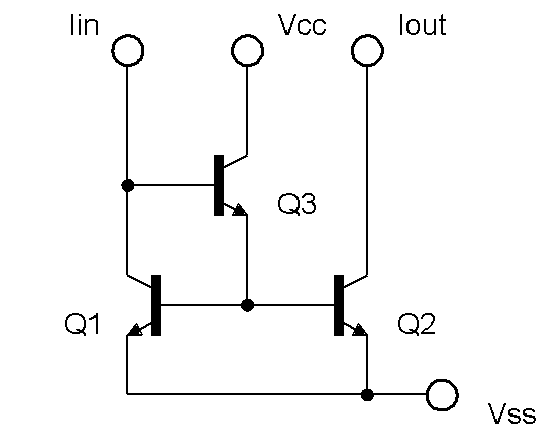
\includegraphics[scale=0.5]{obrazky/ZlepseneWilsonovoZrcadloNPN}
  \end{center}
  \caption[Alenčino zrcadlo]{Zlepšené Wilsonovo proudové zrcadlo.}
\end{figure}

Pro sazbu vektorových obrázků přímo v~\LaTeX{}u je možné doporučit balíček \href{https://www.ctan.org/pkg/pgf}{\texttt{TikZ}}.
Příklady sazby je možné najít na \href{http://www.texample.net/tikz/examples/}{\TeX{}ample}.
Pro vyzkoušení je možné použít programy QTikz nebo TikzEdt.




\chapter{Příklad sazby zdrojových kódů}

\section{Balíček \texttt{listings}}

Pro vysázení zdrojových souborů je možné použít balíček \href{https://www.ctan.org/pkg/listings}{\texttt{listings}}.
Balíček zavádí nové prostředí \texttt{lstlisting} pro sazbu zdrojových kódů, jako například:
%
\begin{lstlisting}[language={[LaTeX]TeX}]
\section{Balíček lstlistings}
Pro vysázení zdrojových souborů je možné použít
	balíček \href{https://www.ctan.org/pkg/listings}%
	{\texttt{listings}}.
Balíček zavádí nové prostředí \texttt{lstlisting} pro
	sazbu zdrojových kódů.
\end{lstlisting}
%
Podporuje množství programovacích jazyků.
Kód k~vysázení může být načítán přímo ze zdrojových souborů.
Umožňuje vkládat čísla řádků nebo vypisovat jen vybrané úseky kódu.
Např.:

\noindent
Zkratky jsou sázeny v~prostředí \texttt{acronym}:
\label{lst:zkratky}
\lstinputlisting[language={[LaTeX]TeX},nolol,numbers=left, firstnumber=6, firstline=6,lastline=6]{text/zkratky.tex}
%
Šířka textu volitelného parametru \verb|KolikMista| udává šířku prvního sloupce se zkratkami.
Proto by měla být zadávána nejdelší zkratka nebo symbol.
Příklad definice zkratky \acs{symfvz} je na výpisu \ref{lst:symfvz}.

\shorthandoff{-}
\lstinputlisting[language={[LaTeX]TeX},frame=single,caption={Ukázka sazby zkratek},label=lst:symfvz,numbers=left,linerange={bsymfvz-\%\%\%\ esymfvz},includerangemarker=false]{text/zkratky.tex}
\shorthandon{-}

\noindent
Ukončení seznamu je provedeno ukončením prostředí:
\lstinputlisting[language={[LaTeX]TeX},nolol,numbers=left,firstnumber=26,linerange=26]{text/zkratky.tex}

\vspace{\fill}

\noindent
{\bf Poznámka k~výpisům s~použitím volby jazyka \verb|czech| nebo \verb|slovak|:}\newline
Pokud Váš zdrojový kód obsahuje znak spojovníku \verb|-|, pak překlad může skončit chybou.
Ta je způsobená tím, že znak \verb|-| je v~českém nebo slovenském nastavení balíčku \verb|babel| tzv.\ aktivním znakem.
Přepněte znak \verb|-| na neaktivní příkazem \verb|\shorthandoff{-}| těsně před výpisem a hned za ním jej vraťte na aktivní příkazem \verb|\shorthandon{-}|.
Podobně jako to je ukázáno ve zdrojovém kódu šablony.


\clearpage

%\section{Výpis kódu prostředí Matlab}
Na výpisu \ref{lst:priklad.vypis.kodu.Matlab} naleznete příklad kódu pro Matlab, na výpisu \ref{lst:priklad.vypis.kodu.C} zase pro jazyk~C.

\lstnewenvironment{matlab}[1][]{%
\iflanguage{czech}{\shorthandoff{-}}{}%
\iflanguage{slovak}{\shorthandoff{-}}{}%
\lstset{language=Matlab,numbers=left,#1}%
}{%
\iflanguage{slovak}{\shorthandon{-}}{}%
\iflanguage{czech}{\shorthandon{-}}{}%
}

\begin{matlab}[frame=single,float=htbp,caption={Příklad Schur-Cohnova testu stability v~prostředí Matlab.},label=lst:priklad.vypis.kodu.Matlab,numberstyle=\scriptsize, numbersep=7pt]
%% Priklad testovani stability filtru

% koeficienty polynomu ve jmenovateli
a = [ 5, 11.2, 5.44, -0.384, -2.3552, -1.2288];
disp( 'Polynom:'); disp(poly2str( a, 'z'))

disp('Kontrola pomoci korenu polynomu:');
zx = roots( a);
if( all( abs( zx) < 1))
    disp('System je stabilni')
else
    disp('System je nestabilni nebo na mezi stability');
end

disp(' '); disp('Kontrola pomoci Schur-Cohn:');
ma = zeros( length(a)-1,length(a));
ma(1,:) = a/a(1);
for( k = 1:length(a)-2)
    aa = ma(k,1:end-k+1);
    bb = fliplr( aa);
    ma(k+1,1:end-k+1) = (aa-aa(end)*bb)/(1-aa(end)^2);
end

if( all( abs( diag( ma.'))))
    disp('System je stabilni')
else
    disp('System je nestabilni nebo na mezi stability');
end
\end{matlab}

\noindent
\begin{minipage}{\linewidth}


%\section{Výpis kódu jazyka C}

\begin{lstlisting}[frame=single,numbers=right,caption={Příklad implementace první kanonické formy v~jazyce C.},label=lst:priklad.vypis.kodu.C,basicstyle=\ttfamily\small, keywordstyle=\color{black}\bfseries\underbar,]
// první kanonická forma
short fxdf2t( short coef[][5], short sample)
{
	static int v1[SECTIONS] = {0,0},v2[SECTIONS] = {0,0};
	int x, y, accu;
	short k;

	x = sample;
	for( k = 0; k < SECTIONS; k++){
		accu = v1[k] >> 1;
		y = _sadd( accu, _smpy( coef[k][0], x));
		y = _sshl(y, 1) >> 16;

		accu = v2[k] >> 1;
		accu = _sadd( accu, _smpy( coef[k][1], x));
		accu = _sadd( accu, _smpy( coef[k][2], y));
		v1[k] = _sshl( accu, 1);

		accu = _smpy( coef[k][3], x);
		accu = _sadd( accu, _smpy( coef[k][4], y));
		v2[k] = _sshl( accu, 1);

		x = y;
	}
	return( y);
}
\end{lstlisting}
\end{minipage}







\chapter{Obsah elektronické přílohy}
Elektronická příloha je často nedílnou součástí semestrální nebo závěrečné práce.
Vkládá se do informačního systému VUT v~Brně ve vhodném formátu (ZIP, PDF\,\dots).

Nezapomeňte uvést, co čtenář v~této příloze najde.
Je vhodné okomentovat obsah každého adresáře, specifikovat, který soubor obsahuje důležitá nastavení, který soubor je určen ke spuštění, uvést nastavení kompilátoru atd.
Také je dobře napsat, v~jaké verzi software byl kód testován (např.\ Matlab 2018b).
Pokud bylo cílem práce vytvořit hardwarové zařízení,
musí elektronická příloha obsahovat veškeré podklady pro výrobu (např.\ soubory s~návrhem DPS v~Eagle).

Pokud je souborů hodně a jsou organizovány ve více složkách, je možné pro výpis adresářové struktury použít balíček \href{https://www.ctan.org/pkg/dirtree}{\texttt{dirtree}}.

\bigskip

{\small
%
\dirtree{%.
.1 /\DTcomment{kořenový adresář přiloženého archivu}.
.2 logo\DTcomment{loga školy a fakulty}.
.3 BUT\_abbreviation\_color\_PANTONE\_EN.pdf.
.3 BUT\_color\_PANTONE\_EN.pdf.
.3 FEEC\_abbreviation\_color\_PANTONE\_EN.pdf.
.3 FEKT\_zkratka\_barevne\_PANTONE\_CZ.pdf.
.3 UTKO\_color\_PANTONE\_CZ.pdf.
.3 UTKO\_color\_PANTONE\_EN.pdf.
.3 VUT\_barevne\_PANTONE\_CZ.pdf.
.3 VUT\_symbol\_barevne\_PANTONE\_CZ.pdf.
.3 VUT\_zkratka\_barevne\_PANTONE\_CZ.pdf.
.2 obrazky\DTcomment{ostatní obrázky}.
.3 soucastky.png.
.3 spoje.png.
.3 ZlepseneWilsonovoZrcadloNPN.png.
.3 ZlepseneWilsonovoZrcadloPNP.png.
.2 pdf\DTcomment{pdf stránky generované informačním systémem}.
.3 student-desky.pdf.
.3 student-titulka.pdf.
.3 student-zadani.pdf.
.2 text\DTcomment{zdrojové textové soubory}.
.3 literatura.tex.
.3 prilohy.tex.
.3 reseni.tex.
.3 uvod.tex.
.3 vysledky.tex.
.3 zaver.tex.
.3 zkratky.tex.
%.2 navod-sablona\_FEKT.pdf\DTcomment{návod na používání šablony}.
.2 sablona-obhaj.tex\DTcomment{hlavní soubor pro sazbu prezentace k~obhajobě}.
%.2 readme.txt\DTcomment{soubor s~popisem obsahu CD}.
.2 sablona-prace.tex\DTcomment{hlavní soubor pro sazbu kvalifikační práce}.
.2 thesis.sty\DTcomment{balíček pro sazbu kvalifikačních prací}.
}
}


\end{document}
